\documentclass[11pt]{article}

\usepackage[margin=1in]{geometry}
\usepackage{amsmath,amssymb}
\usepackage{graphicx}
\usepackage{booktabs}
\usepackage[T1]{fontenc}
\usepackage{lmodern}
\usepackage{microtype}
\usepackage[hidelinks]{hyperref}

\title{Collapsing the dispatch ceiling: kernel fusion for browser-native
WebGPU quantum-circuit simulation}

\author{Ahmet Bar\i{}\c{s} G\"unayd\i{}n\\
\small\textit{Independent researcher\,\textperiodcentered\,github.com/abgnydn/webgpu-q}}

\date{}

\begin{document}
\maketitle

\begin{abstract}
Sequential GPU workloads in the browser are throttled by a fixed per-dispatch
cost: every WebGPU compute dispatch pays a driver/submission overhead that, for
fine-grained work, dominates the actual arithmetic. We quantify this overhead
for browser quantum-circuit simulation --- a per-gate dispatch cost of
$\alpha \approx 5$--$500\,\mu$s on commodity hardware --- and show that
\textbf{kernel fusion}, executing a chain of $k$ quantum gates inside a single
WGSL \texttt{main()}, drives the effective per-gate cost toward $\alpha/k + C$.
We implement fusion as hand-written dense-tile WGSL kernels (2-, 3-, and
4-qubit dense operators) and measure a tier ladder against the simulator's own
unfused multi-dispatch path: brick-wall two-qubit fusion reaches
\textbf{3.04$\times$}, three-qubit-tile (Tier-C) fusion \textbf{4.22$\times$},
both at fidelity $F \ge 0.99999$ vs the unfused statevector. Four-qubit-tile
(Tier-D) fusion is an \textbf{honest negative} --- it tops out at 3.78$\times$
because it crosses from the dispatch-bound into the compute-bound regime, where
the per-block complex-multiply count grows faster than the memory traffic
fusion saves. Fusion is correctness-preserving --- across 360 $(N,k,\text{trial})$
configurations the worst fidelity loss against the unfused statevector is
$1-F = 2.4\times10^{-6}$ --- and pushes the fused statevector update toward
memory-bandwidth-bound throughput. All results run in a browser tab with no
installation; every number is backed by a committed, environment-stamped JSON
artifact. We do not benchmark against native GPU simulators
(cuQuantum~\cite{cuquantum}, Qiskit Aer~\cite{qiskit}) --- those require
hardware unavailable to us --- and position relative to them only through the
bandwidth-fraction argument.
\end{abstract}

\section{Introduction}

A WebGPU compute dispatch is not free. Beyond the shader's own runtime, each
\texttt{dispatchWorkgroups} call pays a driver-side submission and scheduling
cost. For coarse-grained work this is negligible; for \emph{fine-grained,
sequential} work --- where the natural unit of computation is small and many
units run in strict order --- it becomes the dominant term. Quantum-circuit
statevector simulation is a clean instance: each gate is a small ($2\times2$,
$4\times4$) operator applied to a large amplitude array, and gates within a
circuit must be applied in order. A one-gate-per-dispatch scheduler spends more
time in the driver than in the ALUs.

We measure this overhead directly, establish the per-gate cost as a function of
circuit width and fusion factor, and show that fusing gate chains into single
dispatches collapses it. The contribution is not a new simulation algorithm ---
statevector simulation is textbook --- but a quantification of the WebGPU
dispatch ceiling for sequential workloads~\cite{webgpudispatch} and a
fidelity-validated demonstration of how far kernel fusion moves it, including
the regime where fusion stops paying off. Single-kernel fusion has previously
removed this overhead for two other sequential WebGPU workloads --- evolutionary
fitness evaluation, at $159$--$720\times$~\cite{fusionfitness}, and
autoregressive transformer decoding, at $66$--$458\times$~\cite{fusiontransformer}
--- both of which are deeply dispatch-bound. Quantum-circuit statevector
simulation is a third domain, and, as we show, one that reaches
memory-bandwidth saturation early: the same technique that delivers
hundreds-fold speedups on dispatch-bound work caps at a few-fold here. Locating
where a workload sits on that dispatch-bound-to-bandwidth-bound spectrum is the
point. The work runs entirely in a browser tab.

\section{Methods}

\subsection{Simulator and fusion kernels}

Amplitudes are stored as interleaved \texttt{vec2<f32>} (re, im) in a storage
buffer of size $2^{N+3}$ bytes for $N$ qubits. A single-qubit gate dispatches
$N/2$ threads, each updating the amplitude pair that differs in the target bit;
a controlled two-qubit gate dispatches $N/4$ threads. Fusion replaces a chain
of such gates with one dense operator applied in a single dispatch: a
brick-wall layer of adjacent two-qubit gates becomes one dense $4\times4$
dispatch (Tier-B); a three-qubit tile becomes a dense $8\times8$ dispatch
(Tier-C); a four-qubit tile a dense $16\times16$ dispatch (Tier-D). The
dense-tile operators are hand-written WGSL (\texttt{two-qubit-dense.wgsl},
\texttt{three-qubit-dense.wgsl}, \texttt{four-qubit-dense.wgsl}); the fused
operator matrix is precomputed on the host and uploaded once per fused block.
(This is fixed-tile fusion, not a general gate-chain JIT compiler.)

\subsection{Measurement harness}

Wall-clock is measured with \texttt{performance.now()} bracketed by a forced
GPU sync (a mapped readback of a tiny buffer) before and after, because
\texttt{queue.submit} is non-blocking and raw timing is otherwise fiction. Five
warmup samples are discarded and twenty retained; we report the median and flag
any configuration with std/median $> 0.1$ as \texttt{noisy}. Correctness uses
fidelity $F = |\langle\psi_{\mathrm{ref}}|\psi_{\mathrm{test}}\rangle|^2$
against the unfused statevector, with a pass bar of $F \ge 1 - 10^{-5}$ for f32
amplitude paths. Every run emits a JSON artifact recording git SHA,
\texttt{adapter.info}, WebGPU limits, OS, seeds, warmup/trials, and the pass
bar.

\section{Results}

All measurements on an M2 Pro under Chromium with WebGPU.

\subsection{The dispatch ceiling and its collapse}

The per-gate dispatch cost is $\alpha \approx 5$--$500\,\mu$s on commodity
WebGPU (level-1 dispatch-overhead experiment). Fusing $k$ gates per dispatch
drives the effective per-gate cost as $\alpha_{\mathrm{eff}}(k) = \alpha/k + C$:
measured single-qubit chains at $N=8$ fall from $54.5\,\mu$s/gate at $k=1$ to
$17.8\,\mu$s at $k=4$ and $\approx 15.8\,\mu$s at $k=8$, the $1/k$ signature of
amortizing a fixed cost over $k$ operations. (This experiment is flagged
\texttt{noisy} --- sub-$20\,\mu$s timings sit near the harness's sync-fence
resolution --- but the $1/k$ trend is unambiguous across widths.)

\begin{figure}[ht]
  \centering
  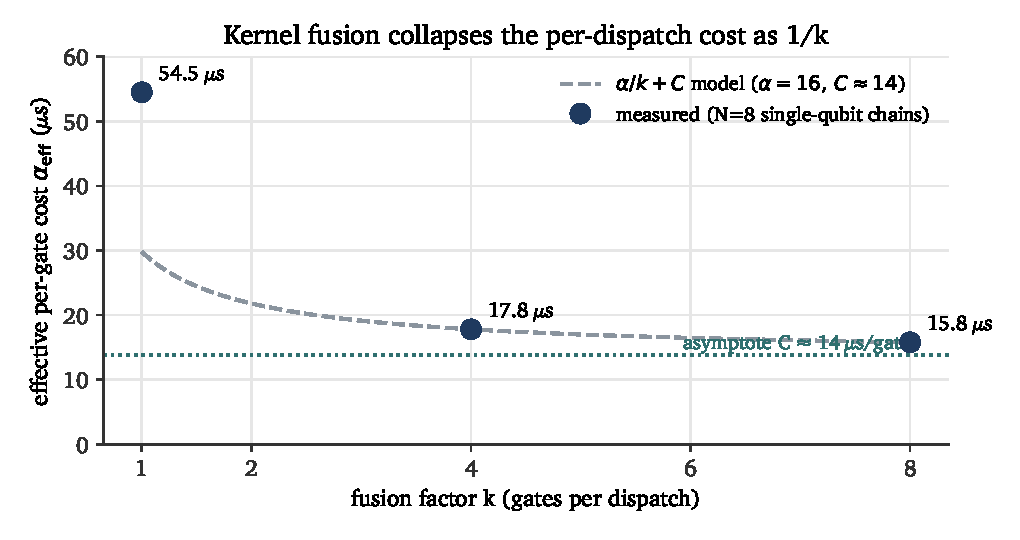
\includegraphics[width=0.82\textwidth]{fig-dispatch.pdf}
  \caption{The per-gate dispatch cost collapses as $1/k$. Measured effective
  per-gate cost for $N{=}8$ single-qubit chains (markers) against the
  $\alpha/k + C$ model (dashed). The cost falls toward a fixed asymptote
  $C\approx14\,\mu$s/gate as the fusion factor $k$ grows; the $k{=}1$ point
  sits above the asymptotic model because the first unfused dispatch carries
  additional fixed submission overhead.}
  \label{fig:dispatch}
\end{figure}

\subsection{Correctness}

Fusion is correctness-preserving. Across 360 $(N, k, \mathrm{trial})$ cells the
worst fidelity is $F = 0.99999762$ ($1 - F = 2.4\times10^{-6}$), inside the
$10^{-5}$ bar; the worst state-norm deviation is $10^{-6}$. Fusion changes
\emph{when} arithmetic happens, not \emph{what} it computes.

\subsection{The fusion tier ladder}

\begin{center}
\resizebox{\textwidth}{!}{%
\begin{tabular}{llllll}
\toprule
tier & fusion & bound & best speedup & worst $F$ & verdict \\
\midrule
B (brick-wall)       & 2-qubit $\to$ dense $4\times4$ & dispatch              & \textbf{3.04$\times$} & 1.0000000 & pass ($\ge2\times$) \\
C (three-qubit tile) & 5 ops $\to$ dense $8\times8$   & dispatch              & \textbf{4.22$\times$} & 0.9999988 & pass ($\ge3\times$) \\
D (four-qubit tile)  & 7 ops $\to$ dense $16\times16$ & dispatch$\to$compute  & 3.78$\times$          & 0.9999995 & \textbf{fail ($\ge5\times$)} \\
\bottomrule
\end{tabular}}
\end{center}

\noindent\footnotesize Best speedups measured at: B --- $N{=}20$, depth $80$;
C --- $N{=}15$, depth $80$; D --- $N{=}20$, depth $80$. \normalsize

\begin{figure}[ht]
  \centering
  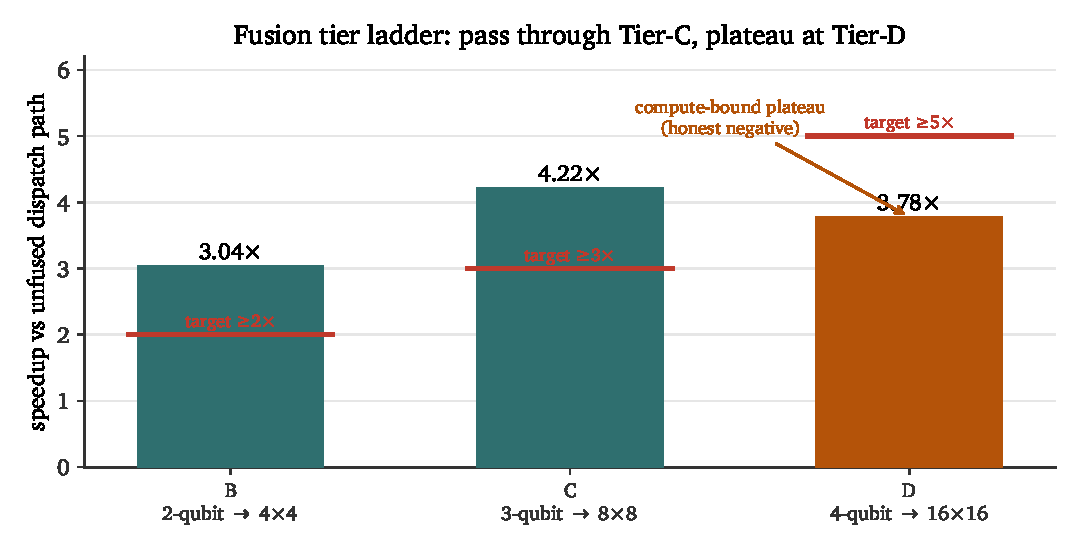
\includegraphics[width=0.82\textwidth]{fig-ladder.pdf}
  \caption{Fusion tier ladder. Brick-wall (B) and three-qubit-tile (C) fusion
  clear their speedup targets; four-qubit-tile (D) fusion plateaus at
  $3.78\times$ against a $5\times$ target because the dense $16\times16$ block
  is compute-bound --- $256$ complex multiplies per $16$-amplitude tile
  ($16$ per amplitude), a $4\times$ growth in per-tile arithmetic over
  Tier-C's $8\times8$ block ($64$ per tile), while the memory traffic fusion
  eliminates grows only $2\times$. The plateau is committed as a
  \texttt{status:"fail"} artifact, not hidden.}
  \label{fig:ladder}
\end{figure}

Tier-D is the informative result. Its correctness is fine (worst
$F = 0.9999995$), but it tops out at 3.78$\times$ against a 5$\times$ target
because the four-qubit dense block performs $256$ complex multiplies per
$16$-amplitude tile ($16$ per amplitude) --- a $4\times$ growth in per-tile
arithmetic over Tier-C's $64$, against only a $2\times$ growth in the memory
traffic that fusion eliminates. Tier-D crosses out of the
dispatch-bound regime into the compute-bound one, where collapsing dispatches
no longer helps. This locates the boundary of the technique rather than hiding
it.

\subsection{Toward bandwidth-bound throughput}

In the dispatch-bound regime (small $N$, long circuits) fused same-qubit chains
at $k=32$ reach 2.62$\times$ ($N=14$, depth 160). As $N$ grows the workload
becomes memory-bandwidth-bound: the fused statevector update's effective
bandwidth rises with $N$ (reaching the hundreds of GB/s range on this device),
and at fixed low depth the fused-vs-unfused speedup compresses toward
1.25$\times$ at $N=20$ (depth 40) --- the expected crossover, since once a
kernel saturates memory bandwidth there is no dispatch overhead left to remove.
At longer depth the dispatch term still dominates and the gain persists (the
$N=20$, depth-160 cell remains $\sim$2.6$\times$). The goal of fusion is to reach
that bandwidth-bound ceiling, not to exceed it.

\section{Honest limitations}

\begin{itemize}
  \item \textbf{Tier-D plateau (\S3.3)} --- fusion past three-qubit tiles is
  compute-bound and does not reach the 5$\times$ target. Committed as a
  \texttt{status:"fail"} artifact with the compute-vs-memory diagnosis.
  \item \textbf{No native-simulator head-to-head.} We measure fusion against
  this simulator's own unfused dispatch path. We did \emph{not} benchmark
  cuQuantum custatevec~\cite{cuquantum} or Qiskit Aer GPU~\cite{qiskit} ---
  both require NVIDIA hardware we do not have --- and we make no head-to-head
  claim against them. Positioning is via the bandwidth-fraction argument only.
  \item \textbf{Fixed-tile fusion, not a JIT chain compiler.} The dense
  operators are hand-written for 2/3/4-qubit tiles; a general gate-chain fuser
  that emits WGSL per circuit is future work.
  \item \textbf{f32 amplitudes} --- the $10^{-5}$ fidelity bar reflects
  single-precision GPU arithmetic; f64 is not available in WebGPU
  1.0~\cite{webgpuspec}.
  \item \textbf{No subgroup operations} --- WebGPU subgroups (shuffle/reduce)
  are out of the 1.0 spec~\cite{webgpuspec}; they would unlock a further
  $\sim$2$\times$ on the reduction-heavy paths when available.
\end{itemize}

\section{Related work}

The per-dispatch overhead of WebGPU is an actively characterized
quantity~\cite{webgpudispatch}. Native GPU statevector simulators --- NVIDIA
cuQuantum custatevec~\cite{cuquantum} and Qiskit Aer GPU~\cite{qiskit} --- are
the performance references for the algorithm, and both are known to approach
memory-bandwidth-bound throughput for long contiguous gate chains; we target
the same bandwidth-fraction regime but in a browser, and do not benchmark
against them directly (\S4). Kernel/operator fusion to amortize launch overhead
is standard in GPU machine-learning runtimes; the contribution here is its
quantification and fidelity-validated application to ordered quantum-gate
chains under the specific constraints of WebGPU~\cite{webgpuspec} in a browser
tab. This is the third domain in which we characterize single-kernel WebGPU
fusion: prior work established the framework for evolutionary fitness
evaluation~\cite{fusionfitness} and autoregressive transformer
decoding~\cite{fusiontransformer}, both deeply dispatch-bound and so reaching
$10^2$--$10^3\times$ speedups. The present domain is the instructive opposite
end of the spectrum --- statevector updates saturate memory bandwidth quickly,
so fusion's payoff is bounded at a few-fold and the Tier-D plateau (\S3.3)
marks the crossover explicitly.

\section{Software availability and reproducibility}

Source: \texttt{github.com/abgnydn/webgpu-q} (MIT). Fusion kernels in
\texttt{src/shaders/} (\texttt{*-dense.wgsl}); experiments in
\texttt{experiments/level-3-fusion/} (E8 correctness, E9 dispatch-collapse, E10
throughput, E11 Tier-B, E12 Tier-C, E13 Tier-D); the committed
\texttt{experiments/results/<date>/level-3/} JSON artifacts are the source of
every number here. No installation: the simulator and its benchmarks run in any
WebGPU-capable Chromium. Each artifact records git SHA, \texttt{adapter.info},
WebGPU device limits, OS, seeds, and the pass bar; timing is sync-fenced;
warmup samples are discarded; failing configurations are committed with a
diagnosis rather than rerun.

\paragraph{Generative-AI disclosure.} Portions of the software, documentation,
and this manuscript were drafted with a large language model used as a coding
and writing aid; all output was author-reviewed, correctness was enforced by
the fidelity tests and committed artifacts, and every quantitative claim is
traceable to a recorded experiment.

\paragraph{Statements.} Sole author; no competing interests; no external
funding. Archived at Zenodo, DOI
\href{https://doi.org/10.5281/zenodo.20494383}{10.5281/zenodo.20494383}.

\section{Conclusion}

WebGPU's per-dispatch overhead caps fine-grained sequential GPU work in the
browser. For quantum-circuit simulation it is $\alpha \approx 5$--$500\,\mu$s/gate,
and kernel fusion drives the effective cost as $\alpha/k + C$: a tier ladder of
dense-tile WGSL kernels delivers up to 4.22$\times$ over the unfused path at
fidelity $\ge 0.99999$, with a clean, documented plateau at four-qubit tiles
where the workload turns compute-bound. The result is a fidelity-validated map
of how far fusion moves the dispatch ceiling --- and exactly where it stops ---
entirely inside a browser tab, with every number reproducible from a URL.

\bibliographystyle{unsrt}
\bibliography{refs-fusion}

\end{document}
